
\chapter{Dropdown}

\section{File Menu}

The file menu contains commands to save the configuration and open/close the console.

\begin{figure}[H]
\centering
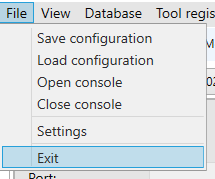
\includegraphics[width=0.3\textwidth]{../Img/Menu_File.PNG}
\caption{File Menu}
\end{figure}

\section{View Menu}

In the view menu you can change the program language as well as display and
hide the register columns of the various tabs as seen in the following image:

\begin{figure}[H]
\centering
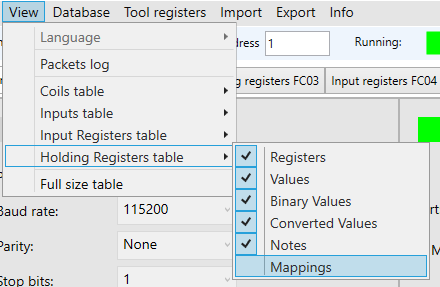
\includegraphics[width=0.6\textwidth]{../Img/Menu_View.PNG}
\caption{View Menu}
\end{figure}

\section{Database Menu}

In the database menu you can create/upload a profile and access the import/export tool of the
profiles. The last menu item "Open temprate editor" opens the window for editing templates
custom templates.

\begin{figure}[H]
\centering
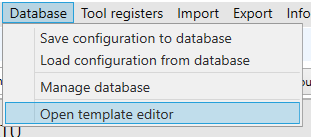
\includegraphics[width=0.45\textwidth]{../Img/Menu_Database.PNG}
\caption{Database Menu}
\end{figure}

\section{Tools Menu}

In the tools menu, command windows can be opened to drive individual bits/bytes/words.

\begin{figure}[H]
\centering
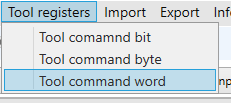
\includegraphics[width=0.32\textwidth]{../Img/Menu_Tools.PNG}
\caption{Tools Menu}
\end{figure}

\section{Import Menu}

In the import menu you can inport a table c
oils or holding registers previously exported
send it send it to the slave. In the case where the registers 
are consecutive you can choose whether to
send them individually (write single coil/write single register) or in bulk 
(write multiple coils/write multiple registers).
It is possible to directly import a csv/json file or
directly import cells copied (ctrl+c) from a spreadsheet
(clipboard).

\begin{figure}[H]
\centering
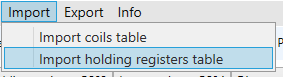
\includegraphics[width=0.4\textwidth]{../Img/Menu_Import.PNG}
\caption{Import Menu}
\end{figure}

\newpage
\section{Export Menu}

In the export menu you can export the tables of the various tabs in csv format.

\begin{figure}[H]
\centering
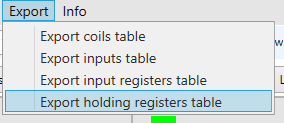
\includegraphics[width=0.4\textwidth]{../Img/Menu_Export.PNG}
\caption{Export Menu}
\end{figure}

\section{Info Menu}

From the info menu you can open this guide, view the program license and
date/build number.

\begin{figure}[H]
\centering
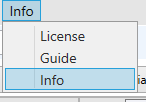
\includegraphics[width=0.25\textwidth]{../Img/Menu_Info.PNG}
\caption{Info Menu}
\end{figure}

In the info window it is possible to read not only the current version but also the date and time of build.

\begin{figure}[H]
\centering
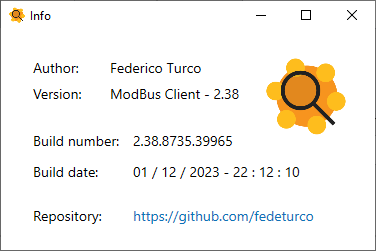
\includegraphics[width=0.5\textwidth]{../Img/Finestra_Info.PNG}
\caption{Info window}
\end{figure}